\subsection{Validierung der Firmware}
\label{subsec:validierung_Firmware}
Die Validierung der Firmware verläuft in verschiedenen Abschnitten. Zuerst werden die Subsysteme, rsp. die einzelnen Klassen (siehe UML-Diagramm Abb. \ref{fig:uml_diagramm}) auf ihre Funktionstüchtigkeit getestet. Diese Validierung wurde meist bereits bei der Implementierung direkt erledigt, wobei grundsätzlich die Daten über die serielle Schnittstelle herausgeschrieben wurden (siehe Kapitel \ref{subsubsec:usbtocomputer} \nameref{subsubsec:usbtocomputer}). Zum Schluss dann nochmals die Firmware als ganzes. Dabei wird überprüft, ob die Klassen richtig miteinander funktionieren.\\

Im Allgemeinen lässt sich sagen, dass es bei aufgetauchten Problemen teils nicht direkt eruieren lässt, ob es ein Firm- oder Hardware Problem ist. Also ist das Troubleshooting recht aufwendig.\\

Bei der Verifikation der Daten der digitalen Sensoren ist die Genauigkeit der Messdaten abhängig der Librarys, mit welchen sie ausgelesen werden. Zusätzlich konnten wir wegen fehlenden Ressourcen keine Referenzmessungen für diese machen.\\

\subsubsection{\_BME280\_}
\label{subsubsec:val_BME280}
\begin{minipage}[b][6.5cm][t]{0.48\textwidth}
Die Datenabfrage des BME280 funktioniert einwandfrei (siehe Abb. \ref{fig:validbme280}). Für die Validierung wurden hier über das Commandlinieinterface die Daten direkt von den Sensoren abgefragt. In der Main selbst können die Daten dann über die Instanz über bme280.setData() gesetzt und dann über die Attribute, welche einen public Access Specifier haben als float Variable ausgelesen werden. Die Abfrage funktionierte im vorherigen Projekt auch schon, wobei in diesem Projekt die Einbindung in die entworfene Hardware realisiert und getestet wurde. Die Daten werden in Grad Celsius, in Prozent (relative Luftfeuchtigkeit) und in hPa angegeben.\\
\end{minipage}
\begin{minipage}[b][6.5cm][t]{0.4\textwidth}
\centering
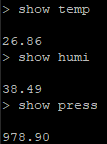
\includegraphics[width=0.9\textwidth]{../../graphics/FW_val/bme280.PNG}
\captionof{figure}{Validierung \_BME280\_}
\label{fig:validbme280}
\end{minipage}

\subsubsection{\_DS3231\_}
\label{subsubsec:valDS3231}
\begin{minipage}[b][6.5cm][t]{0.48\textwidth}
Beim RTC DS3231 können die Zeitdaten abgefragt werden. Wenn die DS3231 aber einmal die Speisung verliert, läuft dieser nicht mehr weiter. Dafür wird dies bei der Initialisierung der Klasse \_DS3231\_ über die Funktion rtc.lostpower() überprüft und falls dies der Fall ist, können die Zeitdaten gleich zu Beginn zurückgesetzt werden (siehe Abb. \ref{fig:validds3231}). In der Abbildung ist zu sehen, dass dieser Vorgang funktioniert. Zusätzlich werden auch die Statusmeldungen herausgeschrieben, dass eine Rücksetzung erforderlich ist.\\
\end{minipage}
\begin{minipage}[b][6.5cm][t]{0.4\textwidth}
\centering
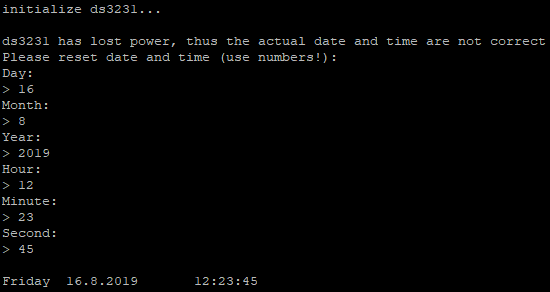
\includegraphics[width=0.9\textwidth]{../../graphics/FW_val/ds3231.PNG} 
\captionof{figure}{Validierung \_DS3231\_}
\label{fig:validds3231}
\end{minipage}

\subsubsection{\_TSL2560\_}
\label{subsubsec:valTSL2560}
\begin{minipage}[b][6.5cm][t]{0.48\textwidth}
Auch hier erfolgt die Abfrage gleich wie beim BME280. Über die Funktion tsl2561.setIlluminance() wird das Attribut von der Main aus gesetzt und dann kann die float Variable illuminance gelesen werden. Die Ausgabe ist in der Abb. \ref{fig:validtsl2561} zu sehen. Die Beleuchtungsstärke ist in lux angegeben. Die Sonnenstunden sind über die gemessene Beleuchtungsstärke eruierbar. Dafür kann der User eine eigene Treshhold definieren bei der Auswertung der Daten.\\
\end{minipage}
\begin{minipage}[b][6.5cm][t]{0.4\textwidth}
\centering
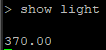
\includegraphics[width=0.5\textwidth]{../../graphics/FW_val/tsl2561.PNG} 
\captionof{figure}{Validierung \_TSL2560\_}
\label{fig:validtsl2561}
\end{minipage}

\subsubsection{\_SIM808\_}
\label{subsubsec:valSIM808}
Hier wird die Funktionstüchtigkeit der Klasse \_SIM808\_ aufgezeigt. Dafür wird in zwei Unterkapitel SMS senden/empfangen und GPS unterteilt. Zu vermerken ist, dass der SIM808 und somit die gesamte Wetterstation ohne gültige SIM-Karte nicht funktioniert. Da diese aber mittlerweile auch bei Pre-Paid-SIM-Karten auf den Namen des Käufers registriert werden, wird diese nicht mit abgegeben.\\
\paragraph{SMS senden/empfangen}
\label{para:validsmssendenempfangen}
\begin{minipage}[b][6.5cm][t]{0.48\textwidth}
Im Loop wird, wie im Kapitel \ref{subsec:uml} erklärt automatisch eine Rückantwort generiert. Um diesem Teil zu verifizieren wurde zweimal eine SMS gesendet. Einmal mit gültigem Command, einmal ohne. In der Abb. \ref{fig:validsim808sms} sind die zurückgesendeten Antworten der Wetterstation zu erkennen. Intern wird dabei die Message und der Sender ausgelesen, ausgewertet und dann an den Sender die entsprechenden Daten zurückgesendet. Zu vermerken ist hier ein Problem, welches nicht gelöst werden konnte. Wenn eine SMS an die Wetterstation gesendet wurde, wird diese in den Platz 1 (Nummer der SMS) des internen Speichers gelegt. Direkt nach dem Rücksenden von der Wetterstation sollte diese empfangene SMS vom User automatisch wieder gelöscht werden, was aber nicht funktioniert. Es muss vorerst noch manuell über das USB-Interface gelöscht werden. Hier müsste also das Fehlerhandling etwas mehr ausgebaut werden, für welche die Zeit durch die aufwendige Hardware leider nicht mehr reichte.\\
\end{minipage}
\begin{minipage}[b][6.5cm][t]{0.4\textwidth}
\centering
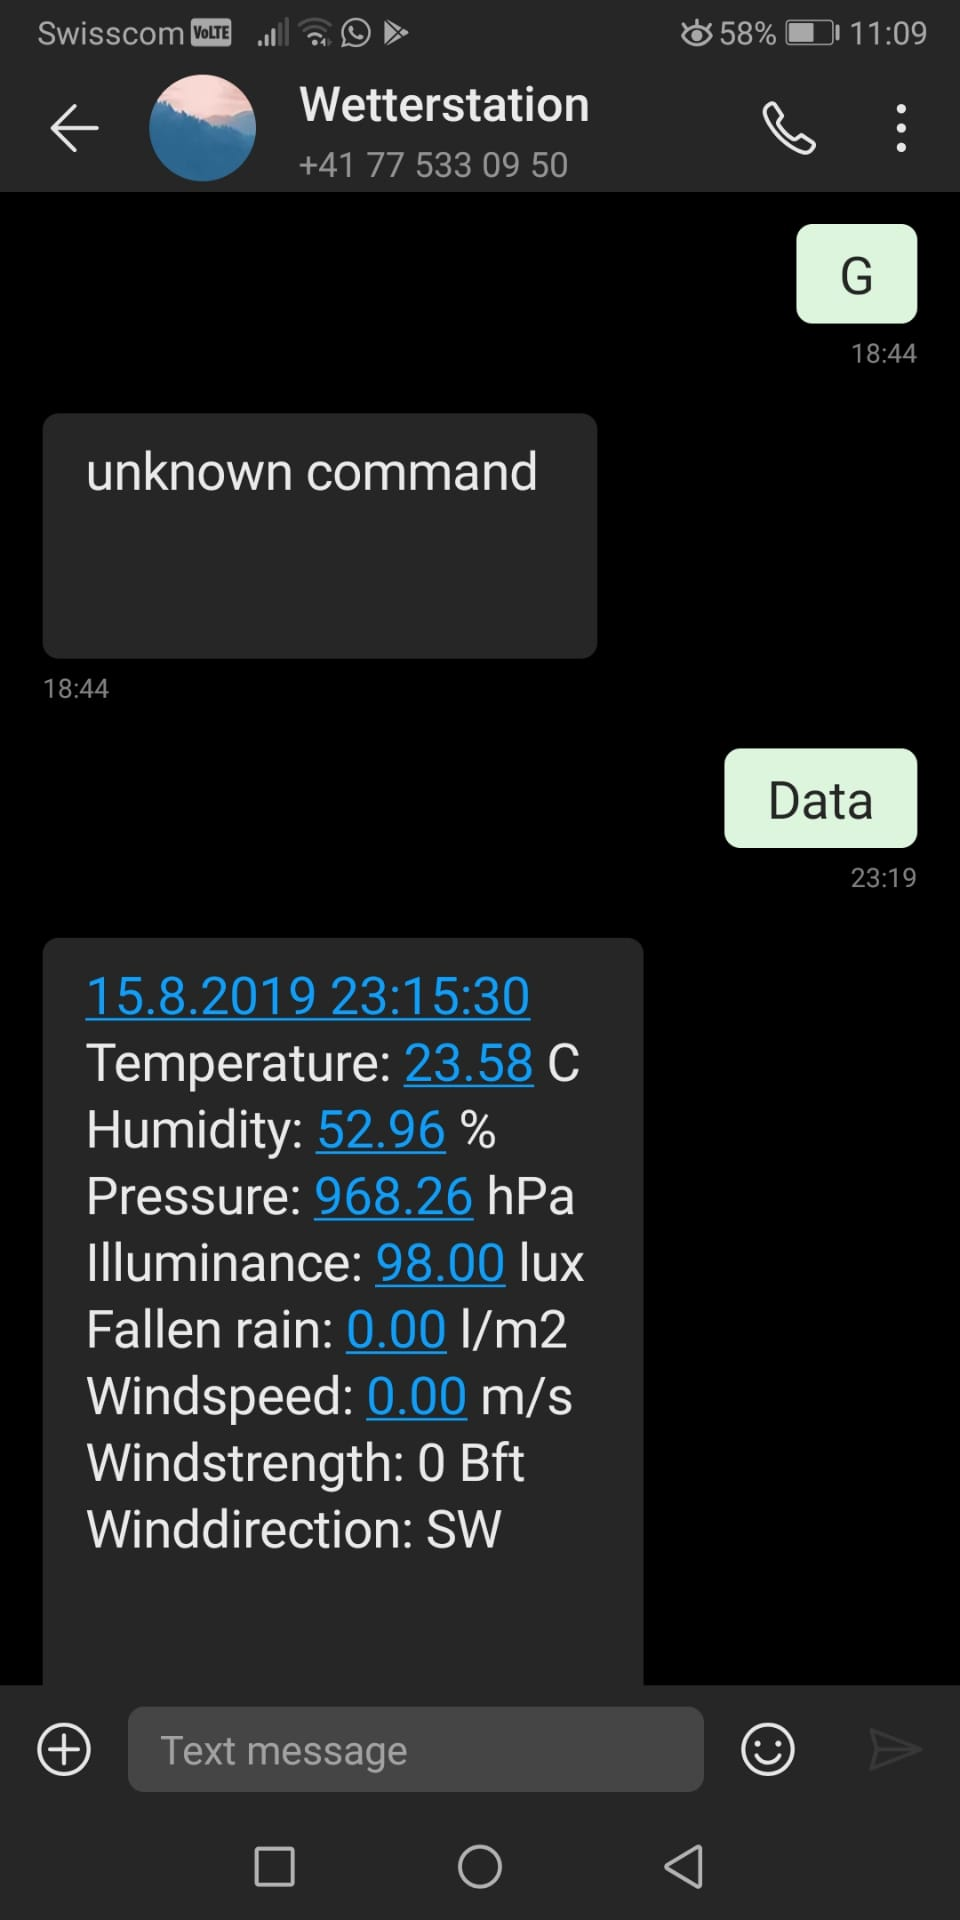
\includegraphics[width=0.9\textwidth]{../../graphics/FW_val/smsantwort.jpeg} 
\captionof{figure}{Validierung \_SIM808\_}
\label{fig:validsim808sms}
\end{minipage}

\paragraph{GPS}
\label{para:validgps}
Für die Verifikation der GPS-Koordinaten wurde lediglich der Command \textit{show gps} im Commandlineinterface ausgeführt. Wenn die Antenne außerhalb eines Gebäudes richtig ausgerichtet wird, können so die Koordinaten von der Mikrocontroller beim SIM808 abgefragt werden. Die Sendeleistung ist leider etwas schwach, weshalb die GPS-Koordinaten nicht immer gleich ausgegeben werden. Dieser Teil wurde vom Gebäude/Raum 4.213 aus beim Fenster getestet. In der Abb. \ref{anfragegps} ist die Anfrage mit der dazugehörigen Antwort der Wetterstation zu sehen.\\
\begin{figure}[h]
\centering
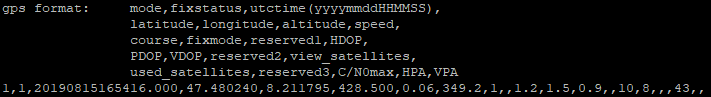
\includegraphics[width=0.6\textwidth]{../../graphics/FW_val/gps_signal.PNG}
\caption{Anfrage GPS-Koordinaten}
\label{fig:anfragegps}
\end{figure}
 Anschließend wurden diese Koordinaten als im Dezimalgrad auf der Website \url{https://www.gpskoordinaten.de} eingetragen. Das Ergebnis des Standorts ist in der Abb. \ref{fig:validgps} zu erkennen. Das Ergebnis scheint auf ca. 10m - 15m genau zu sein.\\
\begin{figure}[h]
\centering
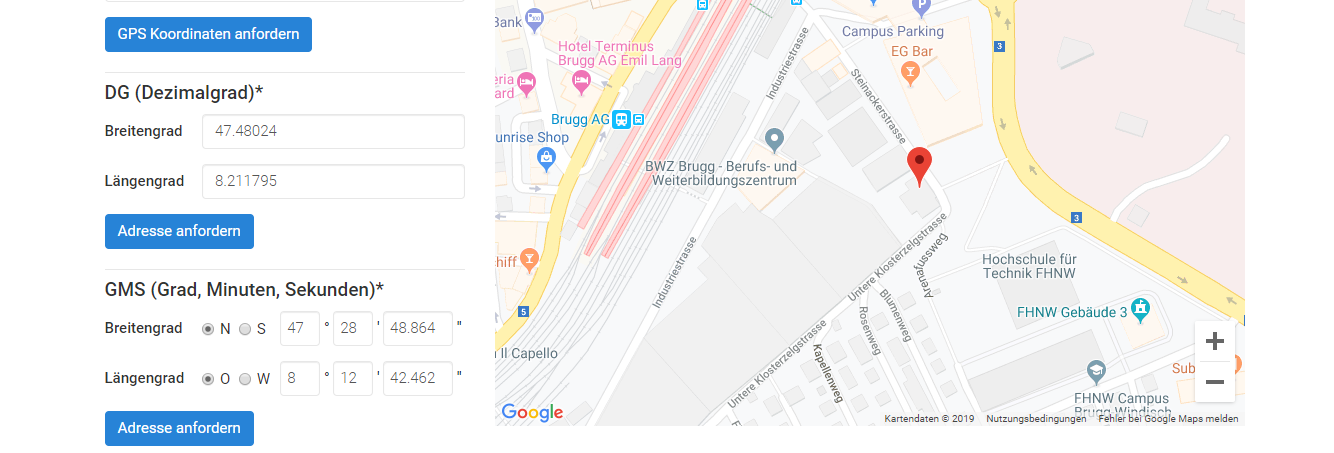
\includegraphics[width=0.7\textwidth]{../../graphics/FW_val/plot_gpsdaten.PNG}
\caption{Verifikation der GPS-Koordinaten}
\label{fig:validgps}
\end{figure}

\subsubsection{CommandLineInterface}
\label{subsubsec:valCommandLineInterface}
Die Klasse CommandLineInterface beinhaltet eine Funktion namens \textit{commandAssignment(String cmd)} über diese werden die vom User eingegebenen Commands den Funktionen zugeordnet. Diese werden über die read() ausgelesen und als String weitergegeben. Diese Klasse funktioniert einwandfrei.\\

\subsubsection{SDCard}
\label{subsubsec:valSDCard}
\begin{minipage}[b][6.5cm][t]{0.48\textwidth}
Bei der Verwendung des Boards wurde eine 16GB $\mu$SD-Karte verwendet. Zur Validierung dieser Klasse kann die Initialisierungsnachrichten im Commandlineinterface betrachtet werden (siehe Abb. \ref{fig:validinitsd}). Dabei kann direkt auf die vorhandene $\mu$SD-Karte zugegriffen werden und dabei relevante Informationen über die Karte herausgeschrieben werden. Zum Initialisierungszeitpunkt traten nie irgendwelche Probleme auf und die Karte konnte immer richtig gelesen werden. In der Abb. \ref{fig:validsdcard} sind ein paar gespeicherte Daten der Wetterstation auf der $\mu$SD-Karte zu sehen. Deutlich zu erkennen ist, dass dies funktioniert. Allerdings traten hier auch wieder Probleme auf, auf welche nicht direkt eine Antwort gefunden werden konnte. Wenn die Messdaten jede Minute gespeichert werden, dann funktioniert dies. Falls die Daten aber all zehnte Minute gespeichert werden sollen, kann die MCU plötzlich keine $\mu$SD-Karte mehr auffinden, obwohl diese nie aus dem Slot entfernt wurde. Es wurde viel Zeit darin investiert, diesen Fehler zu finden, aber wie bereits vorher erwähnt, ist das Troubleshooting aufwendiger, da Fehler beim Layout oder auch bei der Codeabfolge sein kann. Dieser Problem konnte nicht gelöst werden.\\
\end{minipage}
\begin{minipage}[b][6.5cm][t]{0.4\textwidth}
\centering
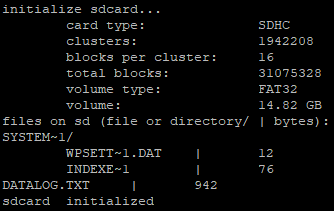
\includegraphics[width=0.9\textwidth]{../../graphics/FW_val/init_sd.PNG}
\captionof{figure}{Initialisierung der $\mu$SD-Karte}
\label{fig:validinitsd}
\centering
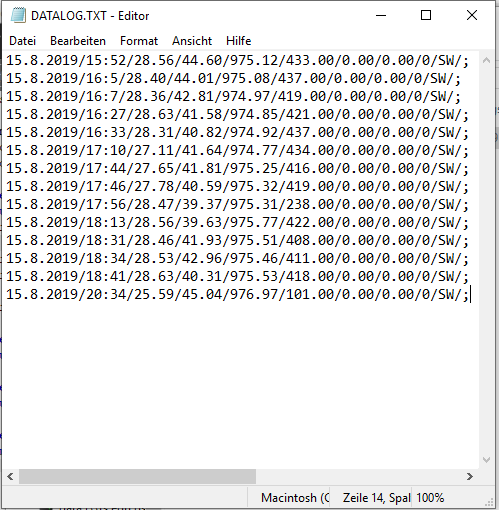
\includegraphics[width=0.9\textwidth]{../../graphics/FW_val/gespeicherteDaten.PNG} 
\captionof{figure}{Validierung SDCard}
\label{fig:validsdcard}
\end{minipage}

\subsubsection{Anemometer, Ombrometer und Windrichtungsgeber}
\label{subsubsec:valaneombrowindr}
Aufgrund von Zeitmangel gegen den Schluss der Arbeit, reichte es nicht, die Firmware, rsp. den Programmcode der Klassen Anemometer, Ombrometer und Windrichtungsgeber nochmals zu überarbeiten. Denn von der im vorherigen Projekt vorhandenen 5V Boardspannung sind es nun nur noch 3.3V. Da das Anemometer und das Ombrometer Flankengetriggert sind, sollte es diese zwei nicht sehr beeinflussen. Allerdings sind nun die Schaltsprünge/-schritte des Windrichtungsgeber kleiner in einem kleineren Spannungsintervall. Darum stimmen hier die in der Firmware implementierten Zuordnungen der Spannunglevels nicht mehr. Für die anderen beiden gilt also noch die Validierung des vorherigen Projekts.\\

\subsubsection{Fazit}
\label{subsubsec:fwfazit}
Auf der Wetterstation befindet sich eine zurzeit funktionierende Firmware. Sie kann SMS auswerten, Daten zurücksenden, Daten speichern, über den Computer über eine serielle Schnittstelle kommunizieren und auch alle relevanten Messdaten erfassen. Im Allgemeinen funktioniert die Wetterstation. Allerdings gibt es drei Hauptprobleme (in den Kapitel \ref{subsubsec:valSIM808}, \ref{subsubsec:valSDCard} und \ref{subsubsec:valaneombrowindr} erklärt) welche die Firmware der Wetterstation unfertig erscheinen lässt. Leider konnte auf diese Probleme nicht mehr eingegangen werden, welche die Wetterstation an ihrer Autonomie hindern.\\